\documentclass{article}
\usepackage[utf8]{inputenc}
\usepackage{amsmath}
\usepackage[magyar]{babel}
\usepackage{amsfonts}
\usepackage{MnSymbol}
\usepackage{wasysym}
\usepackage{graphicx}
\usepackage{tcolorbox}
\usepackage{tikz}
\usetikzlibrary{shapes}

\newcommand\tab[1][1cm]{\hspace*{#1}}


\title{Osztott rendszerek specifikációja és implementációja - dokumentáció}
\author{Lombosi Balázs - D3BA80}
\date{\today}

\begin{document}
\maketitle

\tableofcontents
\newpage

\section{Feladat}

Az egyik bemenet --input\_matrices.txt -- első sorában tartalmazza az $M$ pozitív egész számot, következő $4xM$ sorában pedig az $M$ db $4 x 4$es mátrix sorfolytonos reprezentációját.\\
$M$\\
$x_{1,1,1} \quad x_{1,1,2} \quad x_{1,1,3}\quad x_{1,1,4}$ - az 1. mátrix elemei\\
$x_{1,2,1} \quad x_{1,2,2} \quad x_{1,2,3}\quad x_{1,2,4}$ - $\dots$\\
$x_{1,3,1} \quad x_{1,3,2} \quad x_{1,3,3}\quad x_{1,3,4}$ - $\dots$\\
$x_{1,4,1} \quad x_{1,4,2} \quad x_{1,4,3}\quad x_{1,4,4}$ - az 1. mátrix elemei\\
$\dots\\ $
$x_{M,4,1} \quad x_{M,4,2} \quad x_{M,4,3}\quad x_{M,4,4}$ - az M. mátrix utolsó sorának elemei\\

A másik bemenet --input\_points.txt -- első sorában tartalmazza az $N$ pozitív egész számot, a következő $N$ sorában pedig az $N$ db $3$ hosszú vektorokat.
$N$\\
$v_{1,1} \quad v_{1,2} \quad v_{1,3}$ - az 1. vektor elemei\\
$\dots\\$
$v_{N,1} \quad v_{N,2} \quad v_{N,3}$ - az N. vektor elemei\\

A program olvassa be az adatokat, majd végezze el minden vektorra az $M$ db mátrix szorzást.
Az az eredményt írja az -- output.txt -- kimeneti fájlba.
Megkötés, hogy a fájlból olvasást és a fájlba írást egy szál/folyamat végezze, az egyes mátrix szorzások eredményét pedig egy szál továbbítsa adatcsatornán keresztül egy rákövetkező szálnak.
\newpage

\section{Felhasználói dokumentáció}

\subsection{Környezet}
A program több platformon futtatható, nincsen dinamikus függősége. Telepítésre nincs szükség, elegendő a futtatható állományt elhelyezni a számítógépen \\
(Windows operációs rendszeren \textit{.exe} fájl, UNIX operációs rendszeren \textit{.out} fájl).

\subsection{Használat}
A program használata egyszerű, mert nem vár parancssori paramétereket, így akár parancssoron kívül is lehet futtatni. A fájl mellett kell elhelyezni az \textit{input\_matrices.txt} és \textit{input\_points.txt} fájlokat melyet a program beolvas, az eredményt pedig az \textit{output.txt} nevű fájlba írja.\\
A program futásának feltétele, hogy a bemeneti fájlok \textit{(input\_matrices.txt,input\_points.txt)} felépítése helyes legyen, azaz a feladatban leírtak szerint legyenek benne az adatok.
\newpage

\section{Fejlesztői dokumentáció}
\begin{itshape}
A feladat megoldásához a C++11 es szabványt választottam és annak beépített nyelvi elemeit. \\
\end{itshape}

\subsection{A megoldás módja}
A kódot logikailag több részre bonthatjuk, egy fő- és több alfolyamatra. A főfolyamat, a $main()$ függvény lesz felelős az adatok beolvasásáért az input fájlokból, amik most az \textit{(input\_matrices.txt és input\_points.txt)}. A főfolyamat beolvassa a mátrixokat amikkel a műveleteket fogja elvégezni,majd létrehoz $M+1$ db adatcsatornát és $M$ db szálat, az $M$ db szál mindegyike kap egy-egy mátrixot és azzal a mátrixal fogja elvégezni a szorzást majd továbbítja az eredményt a következő szálnak. A $vektorok$ beolvasásakor az első adatcsatornát ($pipeline$)-t töltjük fel amivel beolvasás közbe már az első szál eltud kezdeni számolni.
\subsection{Implementáció}
A párhuzamosságot a C++11 szabvány nyelvi elemeit kihasználva valósítjuk meg. Az eredmény helyben, a beolvasott vektorban lesz.\\

A C++ beépített adatszerkezeteiből  az adatok tárolásához az $std::vector$-t. A beolvasott mátrixokat egy $std::vector<std::vector<std::vector<int>>>$ adatszerkezetben tároljuk. A főfolyamat létrehoz $M+1$ db adatcsatornát $std::vector<Pipeline<Vector>> pipelines(M+1)$ és $M$ db $threadet$ indít az $Operation$ függvénnyel ami paraméterül kapja az $i$ és $i+1$ -ik adatcsatornát, a threadeket szintén egy $std::vector$ban tároljuk. Ez után a főfolyamat beolvassa a vektorokat a $pipelines[0]$ adatcsatornába.

Az $Operation$ függvény fut az $M$ db szálon, ami induláskor paraméterül kapja a \textit{Mátrixot} amivel a mátrix szorzást végzi, két adatcsatornát ($from, to$), amelyikről olvassa($from$) a vektort amivel el kell végeznie a műveletet, és amelyikre az eredményt kell írnia ($to$), és az $N$ számot, hogy hányszor kell elvégeznie a műveletet azaz hány vektor fog érkezni, a $from$ adatcsatornáról.
\newpage
\subsection{Visszavezetés}
A feladatot vissza vezethetjük az adatcsatorna tételére.
\begin{center}
	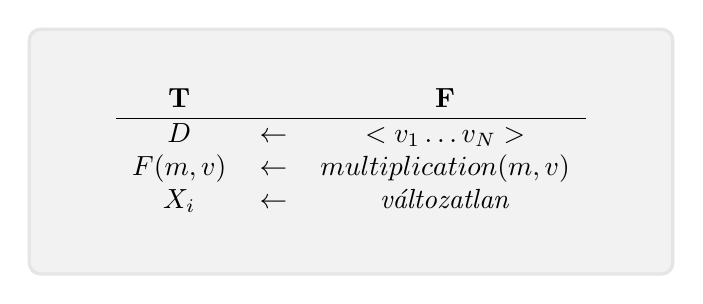
\begin{tikzpicture}
	[mybox/.style={draw=gray!20, fill=gray!10, very thick,
		rectangle, rounded corners, inner sep=30pt, inner ysep=20pt}]
	
	\node [mybox] (box){
		\begin{minipage}{0.50\textwidth}
		\begin{center}
		\begin{tabular}{ccc}
		\textbf{T} &  & \textbf{F} \\ 
		\hline
		$D$ & $\leftarrow$ & $<v_{1} \dots v_{N}>$ \\ 
		$F(m,v)$ & $\leftarrow$ & $multiplication(m,v)$ \\ 
		$X_{i}$ & $\leftarrow$ & \textit{változatlan}\\ 
		\end{tabular} 
		\end{center}
		\end{minipage}
	};
	\end{tikzpicture}
\end{center}
\tab $\forall i \in [0..M]$  $f_{i}(m,v)$ = ($multiplication(m,v)$) 
\subsubsection{Mérések}
\begin{center}
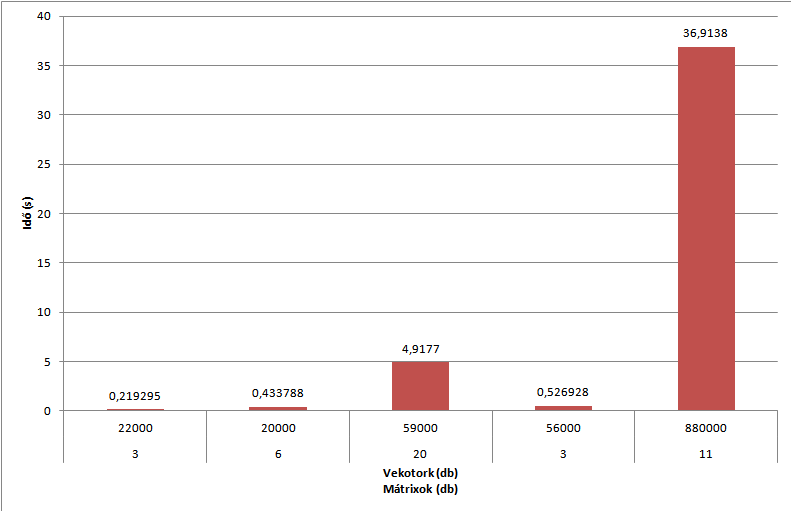
\includegraphics[scale=0.42]{meresek}
\end{center}
\subsection{Fordítás}
A program forráskódja a $main.cpp$ fájlban található.
A program fordításához követelmény egy C++11 szabványt támogató fordítóprogram megléte a rendszeren. A legnépszerűbbek az $msvc$, $g++$ és $clang$.
A fordítás menete (UNIXon g++ 4.9.2-es verziójú fordítóval, Windowson g++ 5.1.0 verziója fordítóval lett tesztelve):
\begin{itemize}
	\item UNIX környezetben a következő: $'g++ \; -std=c++11 \; main.cpp -lpthread'$,
	\item Windows környezetben: $'g++ \; -std=c++11 \; main.cpp'$ .
\end{itemize}
Az $-std=c++11$ kapcsoló szükséges, mert alapértelmezetten egy régebbi C++ szabványt támogat a fordító. UNIX környezetben szükséges a -pthread vagy -lpthread kapcsoló, hogy a fordító tudja, hogy többszálú programot fordít.

\subsection{Tesztelés}
A programot a megadott teszt input fájlokkal teszteltem le. A teszteléshez használt processzor: Intel Core i7-3632QM @ 2.20Ghz .\\

\end {document}